\documentclass[tikz,border=5pt]{standalone}
\usepackage{fontspec}
\setmainfont{Times New Roman}
\usepackage{unicode-math}
\setmathfont{Cambria Math}
\usetikzlibrary{shapes.geometric,shapes.misc,positioning,fit,backgrounds,arrows.meta,calc}

\begin{document}
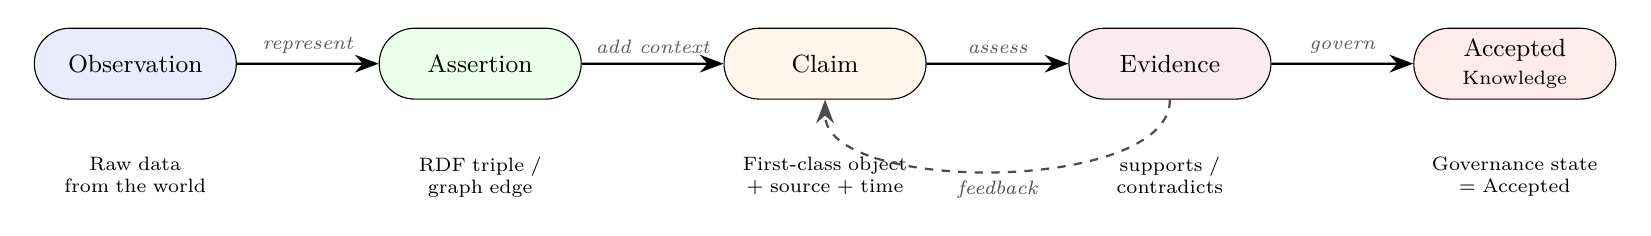
\begin{tikzpicture}[
    node distance=1.2cm and 1.8cm,
    stage/.style={rounded rectangle, draw, minimum width=2.8cm, minimum height=0.9cm, align=center, font=\small},
    arrow/.style={-{Stealth[length=3mm]}, thick},
    label/.style={font=\scriptsize\itshape, text=gray!70!black},
]

% Five stages
\node[stage, fill=blue!8] (obs) {Observation};
\node[stage, fill=green!8, right=of obs] (ast) {Assertion};
\node[stage, fill=orange!8, right=of ast] (clm) {Claim};
\node[stage, fill=purple!8, right=of clm] (evd) {Evidence};
\node[stage, fill=red!8, right=of evd] (acc) {Accepted\\[-1pt]\scriptsize Knowledge};

% Arrows
\draw[arrow] (obs) -- node[label, above] {represent} (ast);
\draw[arrow] (ast) -- node[label, above] {add context} (clm);
\draw[arrow] (clm) -- node[label, above] {assess} (evd);
\draw[arrow] (evd) -- node[label, above] {govern} (acc);

% Annotations below
\node[below=0.6cm of obs, font=\scriptsize, align=center, text width=2.5cm] {Raw data\\from the world};
\node[below=0.6cm of ast, font=\scriptsize, align=center, text width=2.5cm] {RDF triple /\\graph edge};
\node[below=0.6cm of clm, font=\scriptsize, align=center, text width=2.5cm] {First-class object\\+ source + time};
\node[below=0.6cm of evd, font=\scriptsize, align=center, text width=2.5cm] {supports /\\contradicts};
\node[below=0.6cm of acc, font=\scriptsize, align=center, text width=2.5cm] {Governance state\\= Accepted};

% Feedback loop from evidence back to claim
\draw[arrow, dashed, gray!60!black] (evd.south) .. controls +(0,-1.2) and +(0,-1.2) .. (clm.south)
    node[midway, below, font=\scriptsize\itshape, text=gray!60!black] {feedback};

\end{tikzpicture}
\end{document}
